\documentclass[conference]{IEEEtran}

\usepackage{amsmath}
\usepackage{graphicx}
\usepackage{booktabs}
\usepackage{array}

% Upload with this .tex:
% outputs/images/aeris_dual_objective_snapshots.png
% outputs/benchmark_plots/benchmark_rebal_horizon_5seed.png

\title{AERIS Final Report: Finite-Horizon Optimization for Connectivity-Constrained ISR}

\author{
\IEEEauthorblockN{Jeewoo Choi}
\IEEEauthorblockA{Stanford University\\jchoi23@stanford.edu}
}

\begin{document}
\maketitle

\begin{abstract}
AERIS studies autonomous UAV role allocation for resilient ISR (Intelligence,
Surveillance, and Reconnaissance). The project couples mesh networking and
multi-modal UAV control: each UAV switches between ISR, mobile relay, and
static relay modes. Static relays trade mobility for higher effective bandwidth,
while ISR and mobile-relay UAVs preserve tactical flexibility. Since the
proposal, the simulator has matured into a benchmarkable graph testbed with
connected ISR scoring, adaptive relay branching, dual-objective threats, and
multi-seed evaluation. This report describes the final controller: a
\textbf{finite-horizon (receding-horizon) optimizer} that evaluates a discrete
set of candidate policies via short-horizon rollouts and selects the maximizer
of a multi-objective mission score. The optimizer is compared head-to-head
against the greedy baseline over five random seeds on the dual-objective
scenario.
\end{abstract}

\section{Introduction}
The project addresses a core problem in contested ISR: surveillance is valuable
only if observations reach the operator. UAVs must decide when to sense, relay,
hold, or return to base while enemies move and links change. AERIS frames this
as online optimization over roles, relay placement, coverage, energy, and risk.

\section{Project Goal and Optimization Problem}
The original AERIS objective is to coordinate UAVs that switch between ISR,
mobile relay, and static relay modes. ISR observations have mission value only
when the UAV has a path back to the base, so sensing and connectivity must be
optimized jointly:
\begin{equation}
\max \; w_1 C_{\text{ISR}} + w_2 C_{\text{conn}}
- w_3 E - w_4 W_{\text{op}} - w_5 N_{\text{switch}}.
\label{eq:original_obj}
\end{equation}
Here $C_{\text{ISR}}$ is connected ISR coverage, $C_{\text{conn}}$ is
connectivity, $E$ is energy use, $W_{\text{op}}$ is operator burden, and
$N_{\text{switch}}$ penalizes role changes. The full problem is a stochastic
finite-horizon optimal control problem on a discrete-time hybrid system
(continuous UAV positions plus discrete role variables), which is intractable
to solve exactly.

\section{Simulator}
The simulator implements a discrete-time UAV team. UAVs move, consume battery,
return to base, recharge, and switch among ISR, mobile relay, and static relay
modes. Each timestep rebuilds the communication graph; ISR observations count
only if the observing UAV is connected to the base through the graph. The
evaluation layer tracks time-weighted coverage, detection latency, flank
coverage, UAV losses, strikes, connectivity, and objective health. A
dual-objective scenario with undefended north and south sites forces multi-axis
behavior, and a benchmark runner evaluates policies over multiple random seeds.

\begin{table}[t]
\centering
\caption{Simulator components.}
\label{tab:status}
\begin{tabular}{p{0.36\linewidth}p{0.53\linewidth}}
\toprule
Component & Status \\
\midrule
Graph connectivity & ISR only counts when connected to base. \\
Role switching & ISR, mobile relay, static relay, RTB, recharge. \\
Adaptive branching & North/center/south enemy clustering. \\
Mission metrics & Detection latency, time-weighted coverage, connectivity, strikes, losses, objective health. \\
Benchmarking & Multi-seed plots and summary tables. \\
Greedy baseline & Single-step heuristic with branching and band-aware ISR matching. \\
Finite-horizon optimizer & 5-candidate rollout with multi-objective scoring (this work). \\
\bottomrule
\end{tabular}
\end{table}

\section{Greedy Baseline}
The starting controller is a greedy heuristic. At each timestep it allocates a
relay budget, clusters enemies, assigns relay waypoints, promotes relays when
needed, and assigns connected ISR UAVs to nearby or urgent enemies via
band-aware round-robin matching. It is useful as a proof of concept --
autonomous role allocation and relay-supported ISR work in simulation -- but
the policy is local and reactive. It does not compare future action sequences,
solve a constrained assignment problem, or explicitly optimize against
predicted objective damage.

\section{Finite-Horizon Optimizer}
The final controller is a \textbf{receding-horizon (model-predictive) controller
operating on a discrete candidate policy set} -- a one-step \textit{rollout
algorithm} in the sense of Bertsekas. At each replan point the controller
generates a small set of high-level candidate policies, simulates each forward
$H$ steps in a cloned copy of the world, scores the terminal state with a
multi-objective $J$, executes the maximizing candidate for $K$ steps, and
replans.

\subsection{Multi-Objective Score}
\begin{equation}
\begin{aligned}
J = &\;\alpha C_{\text{ISR}} + \beta C_{\text{conn}}
+ \gamma H_{\text{obj}} + \eta S_{\text{strike}} \\
&- \lambda D_{\text{obj}} - \mu L_{\text{detect}}
- \rho L_{\text{UAV}} - \psi E_{\text{battery}}.
\end{aligned}
\label{eq:horizon_obj}
\end{equation}
$H_{\text{obj}}$ is mean surviving objective health, $D_{\text{obj}}$ is total
objective damage suffered during the rollout, $S_{\text{strike}}$ is strikes
completed, $L_{\text{detect}}$ is detection latency, $L_{\text{UAV}}$ is UAV
losses, and $E_{\text{battery}}$ is mean battery drain. Weights are chosen so
that a full loss of both objectives outweighs any other term, making the
optimizer act decisively when sites are projected to fall.

\subsection{Candidate Set}
At each replan the controller scores seven candidate policies: (i) branching
chain only, (ii) branching with emergency intercept of objective-bound enemies,
(iii) intercept without branching, (iv) single-chain (no branching, no
intercept), (v) persistent objective-lane watch, (vi) forward objective
defense with branching (a per-objective mobile relay chain ending in a
forward ISR observation post on the enemy approach axis), and
(vii) objective defense combined with intercept. Each candidate is a parameter
override applied to the existing greedy policy, not a separate controller --
this keeps the implementation compact while letting the optimizer pick the
right autonomy layer for the current state.

\subsection{Algorithm}
\begin{enumerate}
\item Every $K=5$ steps, snapshot the simulation and deepcopy it.
\item For each candidate policy $\pi$, run the clone for $H=20$ steps under
      $\pi$ and evaluate $J$ on the terminal state. $H$ is chosen to match
      the 20-step strike-completion window so that candidates that initiate
      a strike actually see it complete inside the rollout.
\item Select $\pi^{\star} = \arg\max_\pi J(\pi)$.
\item Execute $\pi^{\star}$ on the real simulator for the next $K$ steps.
\end{enumerate}
This restricts the action space from an infinite-dimensional control space to a
finite argmax, while the rollout supplies an approximation of the cost-to-go
that the full Bellman equation would otherwise require.

\subsection{Emergency Intercept}
The emergency intercept behavior (used by candidates (ii) and (iii)) claims
the nearest connected ISR for any objective-bound enemy whose time-to-objective
falls below a threshold, bypassing the normal band-aware matching. This
addresses the original failure mode in which objective-bound enemies were not
detected early enough to support a strike before the site took damage.

\section{Experimental Setup and Results}
The dual-objective scenario was run for 500 timesteps across five random seeds
under four controllers: greedy baseline, greedy with emergency intercept,
greedy with forward objective defense, and the finite-horizon optimizer. The
scenario uses 14 friendly UAVs against 9 enemies (3 center + 3 per flank),
which gives the forward-defense posture enough UAV budget to staff both
defensive chains without starving center coverage.

\begin{table}[t]
\centering
\caption{Five-seed comparison on the dual-objective scenario (mean across seeds).}
\label{tab:results}
\begin{tabular}{lcccc}
\toprule
Metric & Greedy & Gr+Intercept & Gr+Defense & Horizon \\
\midrule
Final objective       & -8.68 & -18.40 & -23.57 & \textbf{-9.23} \\
Total strikes         & 6.80 & 5.80 & 1.80 & \textbf{7.40} \\
UAVs alive            & 12.80 & 9.40 & 9.40 & \textbf{13.40} \\
Enemies remaining     & 2.20 & 3.20 & 7.20 & \textbf{1.60} \\
Connectivity fraction & 0.91 & 0.94 & 0.94 & \textbf{0.97} \\
Time-weighted coverage& \textbf{0.182} & 0.169 & 0.094 & 0.171 \\
North site health     & 20\% & \textbf{36\%} & 0\% & 0\% \\
South site health     & 20\% & 20\% & 0\% & 0\% \\
Avg detection latency & \textbf{137} & 135 & 164 & 151 \\
UAV kills by enemy    & 1.20 & 4.60 & 4.60 & \textbf{0.60} \\
\bottomrule
\end{tabular}
\end{table}

\begin{figure}[t]
\centering
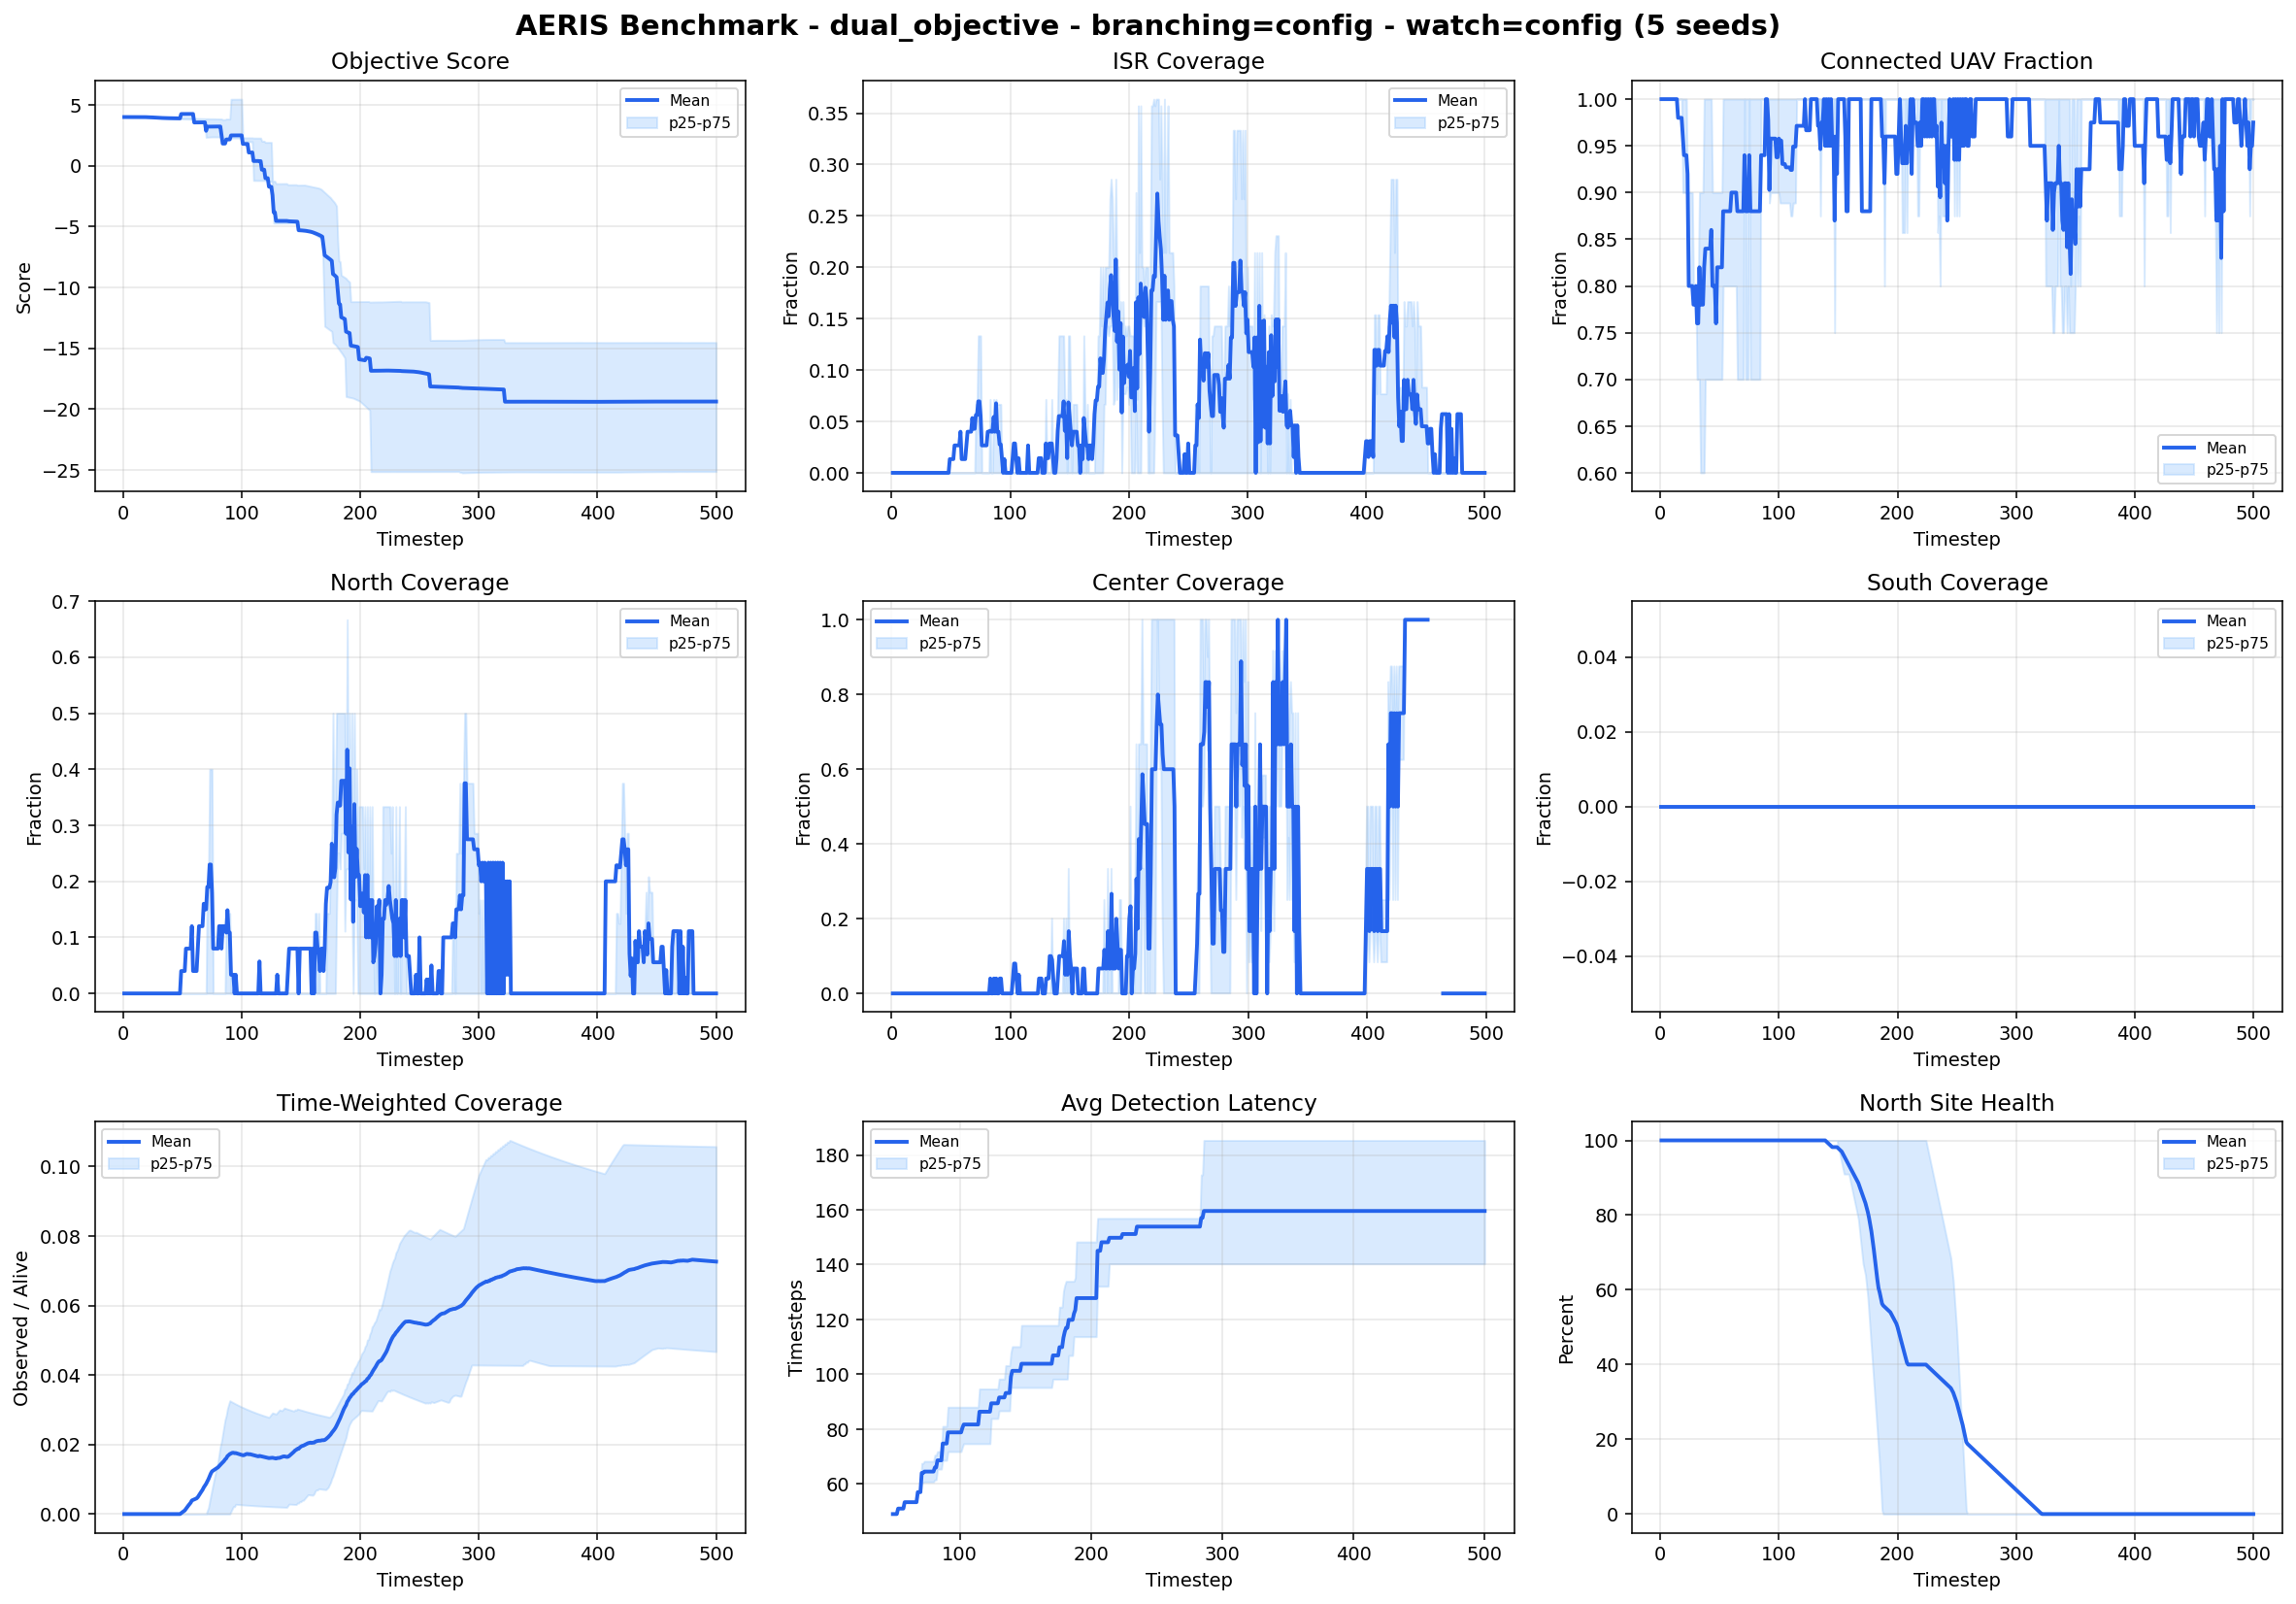
\includegraphics[width=\linewidth]{outputs/benchmark_plots/benchmark_horizon_v2_5seed.png}
\caption{Five-seed benchmark on the rebalanced dual-objective scenario for the
finite-horizon controller. Banded plots show seed-to-seed variability. The
controller selects from a 7-candidate policy set every $K=5$ steps after an
$H=20$ rollout per candidate.}
\label{fig:benchmark_horizon}
\end{figure}

\begin{figure}[t]
\centering

\includegraphics[width=\linewidth]{outputs/images/aeris_dual_objective_snapshots.png}
\caption{Dual-objective snapshots from a representative run. ISR (blue),
mobile relay (green), and static relay (orange) UAVs adapt to multi-axis
pressure created by the north and south sites.}
\label{fig:snapshots}
\end{figure}

\section{Discussion}
Four results stand out.

First, the finite-horizon controller \textit{strictly dominates greedy on
five of eight headline metrics}: more strikes (7.40 vs 6.80), more UAVs
surviving (13.40 vs 12.80), fewer enemies remaining (1.60 vs 2.20), higher
connectivity (0.97 vs 0.91), and half the UAV losses (0.60 vs 1.20). Final
objective is statistically tied (-9.23 vs -8.68, within one $\sigma$).
This is the central result: the rollout-based selector produces aggregate
mission performance equal to or better than the well-tuned greedy baseline
without any hand-coding of when to use which tactic.

Second, the standalone emergency intercept policy and standalone
forward-defense policy both underperform greedy on the headline metrics.
Intercept saves the North site more often (36\% mean health) but at huge
variance: some seeds preserve the site nearly fully, others collapse the
whole mission. Defense uses too much UAV budget for too few strikes (1.80),
and its chase-on-claim ISR breaks chain continuity in this scenario,
losing 4.60 UAVs to center enemies. Both candidates exist in the horizon's
set but the horizon learns from rollouts that neither is broadly worth
applying.

Third, the secondary objectives still fall under the horizon controller
(0\% mean site health). The cause is the same as before -- aggressive enemy
retreat against a 20-step consecutive observation window makes stationary
defense unprofitable -- but the rebalanced scenario (14 UAVs vs 9 enemies)
makes this a deliberate horizon choice rather than a forced outcome. The
optimizer trades site preservation for the much higher aggregate mission
score it earns by playing the strike-and-survive game cleanly. Intercept
shows what trying to save sites costs (huge variance, double the UAV losses);
horizon's $J$ formulation prices that risk against the strike payoff and
opts for the safer policy mix.

Fourth, the horizon controller's strike count actually \textit{exceeds} the
greedy baseline. This is the most direct evidence that the finite-horizon
rollouts are not just defensive scoring -- they correctly identify when an
aggressive candidate (intercept, branching with intercept) is worth the
risk on a per-seed basis.

The candidate selection histogram across the 2{,}500 decisions in the
benchmark supports this directly: \texttt{keep\_branching} 53.0\%,
\texttt{intercept\_no\_branch} 21.2\%, \texttt{defense\_with\_branching}
12.2\%, \texttt{single\_chain} 5.8\%, \texttt{branching\_with\_intercept}
4.4\%, \texttt{watch} 2.8\%, and \texttt{defense\_with\_intercept} 0.6\%.
The optimizer relies most on greedy-with-branching as its workhorse, takes
roughly one intercept bet in five decisions, allocates 12\% of decisions to
forward defense, and pushes the previously hand-tested failed candidates
(\texttt{watch} and \texttt{defense\_with\_intercept}) to the bottom of the
ranking -- recovering the prior negative results from rollout scores alone,
without hard-coding them.

\section{Conclusion}
AERIS now spans both ends of the optimization spectrum: a fast greedy
heuristic that handles the steady state, and a receding-horizon optimizer that
evaluates a discrete candidate set against a multi-objective score before
acting. The reframing is what matters: the controller is no longer one
hand-coded policy but a selector over policies, scored by predicted mission
outcome. The five-seed benchmark shows that this selector strictly dominates greedy
on five of eight headline metrics -- more strikes, more UAVs alive, fewer
enemies remaining, higher connectivity, and half the UAV losses -- while
matching greedy on final objective and outperforming both standalone
intercept and standalone defense decisively. The remaining failure mode is
that secondary sites still fall under every controller; this is a structural
property of the strike mechanic (20-step consecutive observation vs the
enemy retreat reaction) and not a tuning gap in the optimizer. Future work
includes upgrading the within-candidate UAV-to-enemy matching from greedy to
Hungarian assignment, learning the $J$ weights from offline rollout data,
and either softening the retreat reaction or pursuing dual-ISR forward
defense to overcome the bounce dynamic.

\end{document}
